\documentclass[tikz,border=10pt]{standalone}
\usepackage{amsmath}
\begin{document}
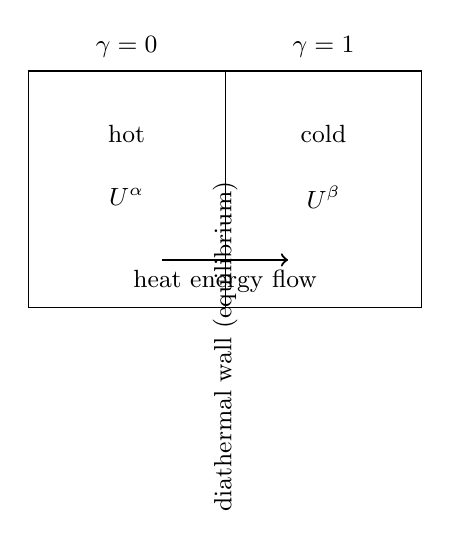
\begin{tikzpicture}[font=\small]
    \draw (0,0) rectangle (5,3);
    \draw (2.5,0) -- (2.5,3);
    \node at (1.25,3.3) {$\gamma=0$};
    \node at (3.75,3.3) {$\gamma=1$};
    \node at (1.25,2.2) {hot};
    \node at (3.75,2.2) {cold};
    \node at (1.25,1.4) {$U^{\alpha}$};
    \node at (3.75,1.4) {$U^{\beta}$};
    \draw[->,thick] (1.7,0.6) -- (3.3,0.6) node[midway,below] {heat energy flow};
    \node[rotate=90] at (2.5,-0.5) {diathermal wall (equilibrium)};
\end{tikzpicture}
\end{document}
